\documentclass{beamer}


% Beamer settings
\usecolortheme{rose}
\beamertemplatenavigationsymbolsempty
\setbeamertemplate{footline}[frame number]

% Packages
\usepackage{amsmath}

\usepackage{pgfplots}
\usepgfplotslibrary{fillbetween}

\usepackage{minted}
\usepackage[T1]{fontenc} % Required by minted to ensure dollar signs are produced instead of pound (sterling) signs

\usepackage{multicol}

\usepackage{booktabs}


\title{A brief introduction to OpenMP}
\subtitle{2: Data sharing clauses}

\begin{document}

\frame{\titlepage}

%-------------------------------------------------------------------------------

\section{Outline}
\begin{frame}
\frametitle{Outline}
\begin{itemize}
  \item Recap
  \item Data sharing clauses
  \item The Pi program
  \item Critical regions
  %\item Atomics
  \item False sharing issues
  \item Reductions
\end{itemize}
\end{frame}
%-------------------------------------------------------------------------------
\section{Recap}
\begin{frame}[fragile]
\frametitle{Recap}
\begin{itemize}
  \item Fork/join execution model.

  \item Shared memory model:
    \begin{itemize}
      \item All threads can read/write the \emph{same} memory.
    \end{itemize}

  \item Set number of threads with \mintinline{bash}|OMP_NUM_THREADS| environment variable.

  \item Parallelise simple loops with worksharing clauses:
  \begin{minted}[frame=single]{c}
  #pragma omp parallel for
  for (int i = 0; i < N; ++i) {
    A[i] = ...;
  }
  \end{minted}

  \item Talked about \mintinline{c}|collapse|, \mintinline{c}|nowait| and \mintinline{c}|schedule| clauses.

\end{itemize}
\end{frame}
%-------------------------------------------------------------------------------

\section{Data sharing}
\begin{frame}
\frametitle{Data sharing}
Remember: OpenMP is a \emph{shared memory} programming model.
\begin{itemize}
  \item By default, all data is available to all threads.
  \item There is a single copy of \emph{shared} data.
\end{itemize}

\vfill

You must specify which data should be \emph{private} to each thread.
\begin{itemize}
  \item Each thread then has local (stack) space for each private variable.
  \item Each copy is only visible to its associated thread.
\end{itemize}

\begin{block}{Notice}
Variables declared \emph{inside} the parallel region will be private to each thread.
\end{block}

\end{frame}


%-------------------------------------------------------------------------------
\begin{frame}
\frametitle{Variables on the heap}
\begin{itemize}
  \item All data on the heap is shared.
  \item Therefore all the data allocated with \mintinline{c}|malloc| is shared.
  \item You must ensure that different threads do not write to the same element of these arrays.
\end{itemize}

\begin{alertblock}{Caution}
Setting a data sharing clause on a heap variable only effects the metadata of the variable.
The pointer could be private, but the target will still be shared.
\end{alertblock}
\end{frame}


%-------------------------------------------------------------------------------
\section{Data clauses}
\begin{frame}
\frametitle{Data clauses}
\begin{itemize}
  \item \mintinline{c}|shared(x)|
    There is one copy of the \mintinline{c}|x| variable. The programmer must ensure synchronisation.
  \item \mintinline{c}|private(x)|
    Each thread gets its own local \mintinline{c}|x| variable. It is not initialised. The value of the original \mintinline{c}|x| variable is undefined on region exit.
  \item \mintinline{c}|firstprivate(x)|
    Each thread gets its own \mintinline{c}|x| variable, and it is initialised to the value of the original variable entering the region.
  \item \mintinline{c}|lastprivate(x)|
    Used for loops. Each thread gets its own \mintinline{c}|x| variable, and on exiting the region the original variable is updated taking the value from the sequentially last iteration.
\end{itemize}

These are the most common clauses that are needed.
\end{frame}

%-------------------------------------------------------------------------------
%\begin{frame}
%\frametitle{Data clauses}
%There is also the \mintinline{c}|threadprivate(x)| directive (not a clause).
%\begin{itemize}
%  \item This says to take a copy of the data in \emph{thread local storage} which is persistent across parallel regions.
%  \item The \mintinline{c}|copyin| directive is a means to initialise \mintinline{c}|threadprivate| data, copying from the master thread.
%\end{itemize}
%
%Unlikely to use this clause.
%Might be useful if using \mintinline{c}|common| blocks (or \mintinline{c}|static| variables in C).
%\end{frame}
%
%-------------------------------------------------------------------------------
\subsection{Private example}
\begin{frame}[fragile]
\frametitle{Private example}
Simple \mintinline{c}|for| loop, which just sets a variable to the iteration number.
Each iteration prints out the current and next value of \mintinline{c}|x|, along with the thread number.
Will see what happens with different data sharing clauses.

\begin{minted}[linenos,breaklines,frame=single, fontsize=\small]{c}
  int x = -1;
  #pragma omp parallel for private(x) / firstprivate(x) / lastprivate(x)
  for (int i = 0; i < N; ++i) {
    printf("Thread %d setting x=%d to %d\n", omp_get_thread_num(), x, i);
    x = i;
  }
\end{minted}
N is set to 10.
Ran using 4 threads.
\end{frame}

%-------------------------------------------------------------------------------
\begin{frame}[fragile]
\frametitle{Private example}
\begin{minted}{bash}
private:
 before: x=-1
  Thread 1 setting x=0 to 3
  Thread 2 setting x=0 to 6
  Thread 3 setting x=0 to 8
  Thread 0 setting x=0 to 0
  Thread 1 setting x=3 to 4
  Thread 2 setting x=6 to 7
  Thread 3 setting x=8 to 9
  Thread 0 setting x=0 to 1
  Thread 1 setting x=4 to 5
  Thread 0 setting x=1 to 2
 after: x=-1
\end{minted}
Each thread starts with its own \mintinline{c}|x|.
No guarantees of initial value, but happened to be zero this time.
\end{frame}

%-------------------------------------------------------------------------------
\begin{frame}[fragile]
\frametitle{Private example}
\begin{minted}{bash}
firstprivate:
 before: x=-1
  Thread 3 setting x=-1 to 8
  Thread 2 setting x=-1 to 6
  Thread 1 setting x=-1 to 3
  Thread 0 setting x=-1 to 0
  Thread 3 setting x=8 to 9
  Thread 2 setting x=6 to 7
  Thread 1 setting x=3 to 4
  Thread 0 setting x=0 to 1
  Thread 1 setting x=4 to 5
  Thread 0 setting x=1 to 2
 after: x=-1
\end{minted}
Each thread starts with its own \mintinline{c}|x|, which set to the value of \mintinline{c}|x| before entering the \mintinline{c}|parallel| region, -1.
\end{frame}

%-------------------------------------------------------------------------------
\begin{frame}[fragile]
\frametitle{Private example}
\begin{minted}{bash}
lastprivate:
 before: x=-1
  Thread 3 setting x=2 to 8
  Thread 2 setting x=1 to 6
  Thread 1 setting x=0 to 3
  Thread 3 setting x=8 to 9
  Thread 0 setting x=-1 to 0
  Thread 2 setting x=6 to 7
  Thread 1 setting x=3 to 4
  Thread 0 setting x=0 to 1
  Thread 1 setting x=4 to 5
  Thread 0 setting x=1 to 2
 after: x=9
\end{minted}
Each thread starts with its own \mintinline{c}|x|, which set to to a garbage value.
On exiting the region, the original \mintinline{c}|x| is set to the value of the last iteration of the loop, 9.
\end{frame}

%-------------------------------------------------------------------------------
%\section{Default data sharing}
%\begin{frame}
%\frametitle{Choosing default data sharing}
%\begin{alertblock}{Note}
%It is especially important to list private variables in Fortran.
%All variables have \emph{global} scope within each \mintinline{fortran}|subroutine| so \emph{everything} is shared by default.
%In C, local scoping rules makes this easier.
%\end{alertblock}
%
%\begin{itemize}
%  \item You can force yourself to specify everything manually by using the \mintinline{fortran}|default(none)| attribute. This is good practice.
%  \item You can also \mintinline{fortran}|default(private)| or \mintinline{fortran}|default(firstprivate)| to make everything private by default --- this might save a lot of typing in an old code with many temporary variables.
%\end{itemize}
%
%\end{frame}

%-------------------------------------------------------------------------------
\section{Calculating Pi}
\begin{frame}
\frametitle{Calculating Pi}
Use a simple program to numerically approximate $\pi$ to explore:
\begin{itemize}
  \item Use of data sharing clauses.
  \item Updating a shared variable in parallel.
  \item Reductions.
\end{itemize}
\end{frame}

%-------------------------------------------------------------------------------
\begin{frame}
\frametitle{Integration to calculate Pi}

$$\int_{0}^{1} \frac{4}{1+x^2} dx = \pi$$

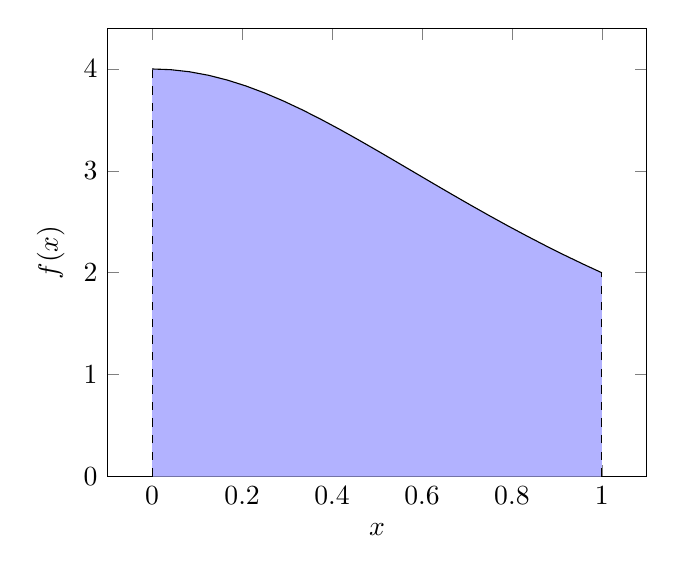
\begin{tikzpicture}
  \begin{axis}[xlabel={$x$},ylabel={$f(x)$},ymin=0]
    \addplot [name path=A, domain=0:1] {4/(1+x*x)};
    \addplot[dashed] coordinates {(0,0) (0,4)};
    \addplot[dashed] coordinates {(1,0) (1,2)};
    \path [name path=axis] (axis cs:0,0) -- (axis cs:1,0);
    \addplot[blue!30] fill between [of=A and axis, domain=0:1];
  \end{axis}
\end{tikzpicture}
\end{frame}

%-------------------------------------------------------------------------------
\begin{frame}
\frametitle{Trapezoidal rule}
Sum the area of the boxes. Choose a small \emph{step} size to generate lots of boxes, and increase accuracy.
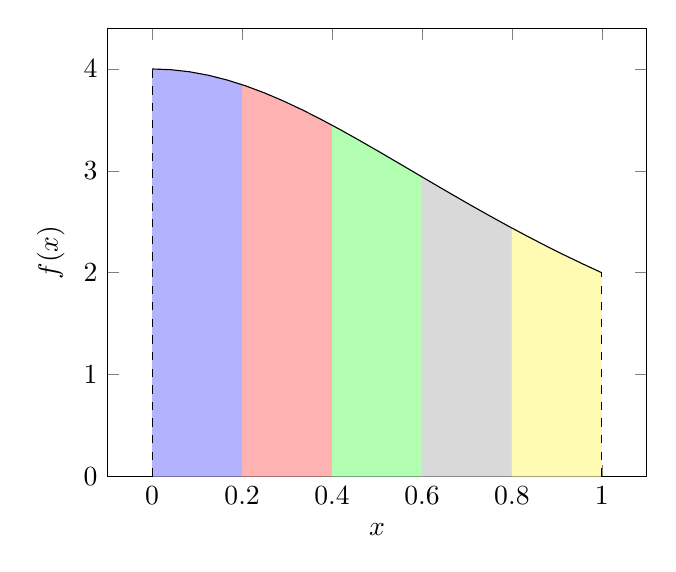
\begin{tikzpicture}
  \begin{axis}[xlabel={$x$},ylabel={$f(x)$},ymin=0]
    \addplot [name path=A, domain=0:1] {4/(1+x*x)};
    \addplot[dashed] coordinates {(0,0) (0,4)};
    \addplot[dashed] coordinates {(1,0) (1,2)};
    \path [name path=axis] (axis cs:0,0) -- (axis cs:1,0);
    \addplot[blue!30] fill between [of=A and axis, soft clip={domain=0:0.2}];
    \addplot[red!30] fill between [of=A and axis, soft clip={domain=0.2:0.4}];
    \addplot[green!30] fill between [of=A and axis, soft clip={domain=0.4:0.6}];
    \addplot[gray!30] fill between [of=A and axis, soft clip={domain=0.6:0.8}];
    \addplot[yellow!30] fill between [of=A and axis, soft clip={domain=0.8:1}];
  \end{axis}
\end{tikzpicture}
\end{frame}

%-------------------------------------------------------------------------------
\begin{frame}[fragile]
\frametitle{Code}
We will use this code which calculates the value of $\pi$ as an example for the remainder of this session.

\begin{minted}[linenos,breaklines,frame=single]{c}
  double step, x, sum, pi;
  step = 1.0/num_steps;
  for (int ii = 1; ii <= num_steps; ++ii) {
    x = (ii-0.5)*step;
    sum = sum + (4.0/(1.0+x*x));
  }
  pi = step * sum;
\end{minted}

With 100,000,000 steps, this takes 0.368s on my laptop.

%Full implementation: \mintinline{bash}|pi.f90|.
\end{frame}

%-------------------------------------------------------------------------------
\begin{frame}[fragile]
\frametitle{Parallelising the loop}

Use a worksharing directive to parallelise the loop.

\begin{minted}[linenos,breaklines,frame=single]{c}
  double step, x, sum, pi;
  step = 1.0/num_steps;
  #pragma omp parallel for private(x)
  for (int ii = 1; ii <= num_steps; ++ii) {
    x = (ii-0.5)*step;
    sum = sum + (4.0/(1.0+x*x));
  }
  pi = step * sum;
\end{minted}

\vfill

What about data sharing?
\begin{itemize}
  \item \mintinline{c}|x| needs to be used independently by each thread, so mark as \mintinline{c}|private|.
  \item \mintinline{c}|sum| needs to be updated by \emph{all} threads, so leave as \mintinline{c}|shared|.
\end{itemize}

\end{frame}

%-------------------------------------------------------------------------------
\section{Critical regions}
\begin{frame}[fragile]
\frametitle{Parallelising with critical}
\begin{itemize}
  \item But need to be careful changing the \mintinline{c}|shared| variable, \mintinline{c}|sum|.
  \item All threads can update this value directly!
  \item A \mintinline{c}|critical| region only allows one thread to execute at any one time. No guarantees of ordering.
\end{itemize}

\begin{minted}[linenos,breaklines,frame=single]{c}
  double step, x, sum, pi;
  step = 1.0/num_steps;
  #pragma omp parallel for private(x)
  for (int ii = 1; ii <= num_steps; ++ii) {
    x = (ii-0.5)*step;
    #pragma omp critical
    {
    sum = sum + (4.0/(1.0+x*x));
    }
  }
  pi = step * sum;
\end{minted}

\end{frame}

%%-------------------------------------------------------------------------------
%\begin{frame}
%\frametitle{Runtimes}
%Run on a MacBook Pro (Intel Core i7-4980HQ CPU @ 2.80GHz) with 4 threads.
%
%\vfill
%
%\begin{table}
%\begin{tabular}{cc}
%\toprule
%Implementation & Runtime (s) \\
%\midrule
%Serial   & 0.368 \\
%Critical & 426.1 \\
%\bottomrule
%\end{tabular}
%\end{table}
%
%%Full implementation: \mintinline{bash}|pi_critical.f90|.
%
%\begin{center}
%\large Really slow!
%\end{center}
%
%\end{frame}
%
%%-------------------------------------------------------------------------------
%\section{Atomics}
%\begin{frame}[fragile]
%\frametitle{Atomics}
%A \mintinline{fortran}|critical| region protects a whole block of code. For a single operation, can use \mintinline{fortran}|atomic| instead.
%
%Atomic operations are with respect to the memory access of a scalar variable {\tt x}.
%
%\begin{itemize}
%  \item \mintinline{fortran}|read| for \mintinline{fortran}|v = x|
%  \item \mintinline{fortran}|write| for \mintinline{fortran}|x = expr|
%  \item \mintinline{fortran}|update| for \mintinline{fortran}|x = x op expr|
%  \item \mintinline{fortran}|capture| for read and write/update. The result is retained: \mintinline{fortran}|x = x op expr; v = x|
%\end{itemize}
%
%Not specifying an atomic clause defaults to \mintinline{fortran}|update|.
%\end{frame}
%
%%-------------------------------------------------------------------------------
%\begin{frame}[fragile]
%\frametitle{Atomic pi}
%\begin{minted}[linenos,breaklines]{fortran}
%  step = 1.0/num_steps
%  !$omp parallel do private(x)
%  do ii = 1, num_steps
%    x = (ii-0.5)*step
%    !$omp atomic
%    sum = sum + (4.0/(1.0+x*x))
%  end do
%  !$omp end parallel do
%  pi = step * sum
%\end{minted}
%\end{frame}
%
%-------------------------------------------------------------------------------
\begin{frame}
\frametitle{Runtimes}
Run on a MacBook Pro (Intel Core i7-4980HQ CPU @ 2.80GHz) with 4 threads.

\vfill

\begin{table}
\begin{tabular}{cc}
\toprule
Implementation & Runtime (s) \\
\midrule
Serial   & 0.368 \\
Critical & 426.1 \\
Atomic   & 8.3 \\
\bottomrule
\end{tabular}
\end{table}

%Full implementation: \mintinline{bash}|pi_atomic.f90|.

\begin{center}
\large Slower than serial!
\end{center}

\end{frame}

%-------------------------------------------------------------------------------
\section{Avoiding critical regions}
\begin{frame}
\frametitle{Independent summation}
\begin{itemize}
  \item Criticals or atomics methods cause threads to synchronise for every update to \mintinline{c}|sum|.
  \item But each thread could compute a partial sum independently, synchronising once to total at the end.
\end{itemize}

\vfill

Make \mintinline{c}|sum| an array of length equal to the number of threads.
\begin{itemize}
  \item Each thread stores its partial sum, and the array is totalled by the master thread serially at the end.
  \item As it's \emph{shared memory}, the \mintinline{c}|sum| array can be read just fine on the master rank.
\end{itemize}
\end{frame}

%-------------------------------------------------------------------------------
\begin{frame}[fragile]
\frametitle{Independent summation}
\begin{minted}[linenos,breaklines,frame=single]{c}
  step = 1.0/num_steps;
  #pragma omp parallel private(x,tid)
  {
  tid = omp_get_thread_num();
  sum[tid] = 0.0;
  #pragma omp for
  for (int ii = 1; ii <= num_steps; ++ii) {
    x = (ii-0.5)*step;
    sum[tid] = sum[tid] + (4.0/(1.0+x*x));
  }
  }
  for (int ii = 0; ii < nthreads; ++ii) {
    pi = pi + sum[ii];
  }
  pi = pi * step;
\end{minted}
\end{frame}

%-------------------------------------------------------------------------------
\begin{frame}
\frametitle{Runtimes}
Run on a MacBook Pro (Intel Core i7-4980HQ CPU @ 2.80GHz) with 4 threads.

\vfill

\begin{table}
\begin{tabular}{cc}
\toprule
Implementation & Runtime (s) \\
\midrule
Serial   & 0.368 \\
Critical & 426.1 \\
Atomic   & 8.3 \\
Array    & 2.8* \\
\bottomrule
\end{tabular}
\end{table}

%Full implementation: \mintinline{bash}|pi_array.f90|.
* Might be faster if have a smart compiler which avoided false sharing.

\begin{center}
\large Fastest parallel version so far, but still slow.
\end{center}

\end{frame}

%-------------------------------------------------------------------------------
\section{False sharing}
\begin{frame}
\frametitle{False sharing}
\begin{columns}
\begin{column}{.65\textwidth}
This code is susceptible to \emph{false sharing}.
\begin{itemize}
  \item False sharing occurs when different threads update data on the same cache line.
  \item It is a \emph{different} phenomenon to cache thrashing, as result of parallel shared memory execution.
  \item Cache system is coherent between cores, so data consistency must be maintained.
  \item The cache line is no longer up to date because another thread changed it (in their local cache).
  \item Therefore, cache line must be flushed to memory and reread into the other thread every time.
\end{itemize}
\end{column}
\begin{column}{.35\textwidth}
\begin{center}
\includegraphics[width=\textwidth]{intel_false_sharing.png}
\end{center}
\end{column}
\end{columns}
{\Tiny \url{https://software.intel.com/en-us/articles/avoiding-and-identifying-false-sharing-among-threads}}
\end{frame}

%-------------------------------------------------------------------------------
%\begin{frame}
%\frametitle{Flush}
%\begin{itemize}
%  \item The \mintinline{fortran}|flush()| construct ensures that the variables are consistent between the thread's memory and main memory.
%  \item Don't want to go into complicated parts of the OpenMP memory model.
%  \item In general, don't need to worry about this stuff.
%  \item Without the flush, the write to memory will be lowered to after the loop, so false sharing only occurs once at the end.
%  \item Here we use it to \emph{ensure} that false sharing occurs every time to highlight the performance hit.
%\end{itemize}
%\end{frame}
%
%-------------------------------------------------------------------------------
\begin{frame}[fragile]
\frametitle{Firstprivate pi}
Can use data sharing clauses to our advantage here:

Give each thread a \emph{scalar} copy of \mintinline{c}|sum| to compute their partial sum, and reduce with only one critical (or atomic) region at the end.
No false sharing, as value is just a single number (i.e.\ a register).
\begin{minted}[linenos,breaklines,frame=single,fontsize=\small]{c}
  step = 1.0/num_steps;
  #pragma omp parallel private(x) firstprivate(sum)
  {
  #pragma omp for
  for (int ii = 1; ii <= num_steps; ++i) {
    x = (ii-0.5)*step;
    sum = sum + (4.0/(1.0+x*x));
  }
  #pragma omp critical
  pi = pi + sum;
  }
  pi = pi * step;
\end{minted}
\end{frame}

%-------------------------------------------------------------------------------
\begin{frame}
\frametitle{Runtimes}
Run on a MacBook Pro (Intel Core i7-4980HQ CPU @ 2.80GHz) with 4 threads.

\vfill

\begin{table}
\begin{tabular}{cc}
\toprule
Implementation & Runtime (s) \\
\midrule
Serial        & 0.368 \\
Critical      & 426.1 \\
Atomic        & 8.3 \\
Array         & 2.8 \\
First private & 0.104 \\
\bottomrule
\end{tabular}
\end{table}

%Full implementation: \mintinline{bash}|pi_private.f90|.

\begin{center}
\large Finally faster than serial! Around 3.5X faster on 4 threads.
\end{center}

\end{frame}

%-------------------------------------------------------------------------------
\section{Reductions}
\begin{frame}[fragile]
\frametitle{Reductions}
Much simpler to use the OpenMP \mintinline{c}|reduction| clause on a worksharing loop.
Specify the operation and the variable.
\begin{multicols}{2}
\begin{itemize}
  \item \mintinline{c}{reduction(+:var)}
  \item \mintinline{c}{reduction(-:var)}
  \item \mintinline{c}{reduction(*:var)}
  \item \mintinline{c}{reduction(&&:var)}
  \item \mintinline{c}{reduction(||:var)}
  \item \mintinline{c}{reduction(^:var)}
  \item \mintinline{c}{reduction(&:var)}
  \item \mintinline{c}{reduction(|:var)}
  \item \mintinline{c}{reduction(min:var)}
  \item \mintinline{c}{reduction(max:var)}
\end{itemize}
\end{multicols}

Can also do array reductions. Each element of array is treated as own, separate, reduction.
Similar to:
\begin{minted}[breaklines]{c}
MPI_Allreduce(MPI_IN_PLACE, arr, N, MPI_DOUBLE, MPI_SUM, 0, MPI_COMM_WORLD);
\end{minted}

\end{frame}

%-------------------------------------------------------------------------------
\begin{frame}[fragile]
\frametitle{Pi reduction}
Much simpler to write using the \mintinline{c}|reduction| clause --- just need a single directive:
\begin{minted}[linenos,breaklines,frame=single]{c}
  step = 1.0/num_steps;
  #pragma omp parallel for private(x) reduction(+:sum)
  for (int ii = 1; ii <= num_steps; ++i) {
    x = (ii-0.5)*step;
    sum = sum + (4.0/(1.0+x*x));
  }
  pi = step * sum;
\end{minted}

%Full implementation: \mintinline{bash}|pi_reduction.f90|.
\end{frame}

%-------------------------------------------------------------------------------
\begin{frame}
\frametitle{Runtimes}
Run on a MacBook Pro (Intel Core i7-4980HQ CPU @ 2.80GHz) with 4 threads.

\vfill

\begin{table}
\begin{tabular}{cc}
\toprule
Implementation & Runtime (s) \\
\midrule
Serial        & 0.368 \\
Critical      & 426.1 \\
Atomic        & 8.3 \\
Array         & 2.8 \\
First private & 0.104 \\
Reduction     & 0.095 \\
\bottomrule
\end{tabular}
\end{table}

\vfill

Around 3.9X faster on 4 threads!

\vfill


\begin{block}{Recommendation}
Use the \mintinline{c}|reduction| clause for reductions.
\end{block}

\end{frame}

%-------------------------------------------------------------------------------
%\section{Exercise}
%\begin{frame}
%\frametitle{Exercise}
%\begin{itemize}
%  \item Start with your parallel 5-point stencil code from last time.
%  \item Change the code to print out the total of the cells (excluding halo) every timestep.
%  \item You'll need to implement a parallel reduction to do this.
%  \item Try the different techniques shown to implement reductions:
%    \begin{itemize}
%      \item Critical sections.
%      \item Atomics.
%      \item Reduction clause.
%    \end{itemize}
%  \item Extension: there is also a Jacobi code to parallelise --- it needs a reduction too.
%\end{itemize}
%\end{frame}
%
%%-------------------------------------------------------------------------------
\begin{frame}
\frametitle{Summary}
\begin{itemize}
  \item Have now covered the most common parts of OpenMP.
  \item 80/20 rule: Most programs will only use what you know so far.
  %\item In the remaining sessions you'll learn to program OpenMP well on modern computer architecture.
  \item OpenMP is deceptively simple!
\end{itemize}
\end{frame}

%-------------------------------------------------------------------------------
\end{document}
